\chapter{Introduction}
The Backlog and Traceability document presents all the customer needs and requirements. It describes how Scrum is implemented and how User Stories are utilized. This document also provides an overview of the User Stories and Tasks related to the project and how traceability is ensured. \\

JIRA Project Management tool is used to facilitate the project and to keep track of all tasks and resources. JIRA provides some useful features such as Sprint Health seen in Fig. \ref{fig:sh} and Burndown charts seen in Fig. \ref{fig:bdc}. All the activities have a unique JIRA ID.\\
 

\begin{figure}[h]
        \centering
         \begin{minipage}[b]{0.3\textwidth}
            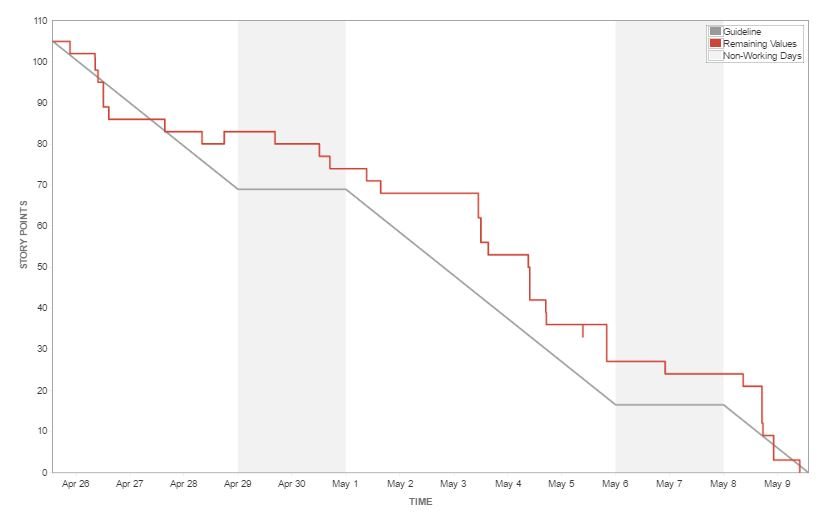
\includegraphics[width = 1\textwidth]{VAPIQ-PICTURES/BDSprint8}
            \caption{Burndown Chart}
            \label{fig:bdc}
        \end{minipage}
        \hfill
        \begin{minipage}[b]{0.6\textwidth}
            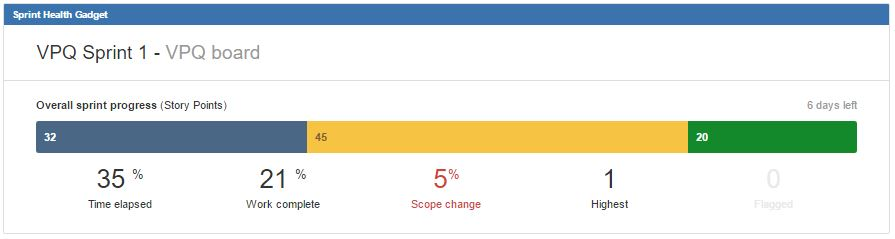
\includegraphics[width = 1\textwidth]{VAPIQ-PICTURES/SH}
            \caption{Sprint Health}
            \label{fig:sh}
        \end{minipage}
\end{figure}


\vspace*{1cm}

%The project dependent on an external tracking system, located at KONGSBERG Innovation Center (KIC), named Qualisys. This is a motion tracking system which uses small reflective bullets to track the motion and position of the object they are placed on. By using this system, we should be able to create reproducible test results. We are going to write our own flight controller using real-time data received from Qualisys. 

